%@COPYRIGHT VOLLMAIER ALOIS
\definecolor{hellgrau}{RGB}{230, 230, 230}
\lohead{Vollmaier Alois}
\chapter{Informatik}\label{ch:informatik}

\section{Allgemeines}\label{sec:einleitung}
Im folgenden Projektteil werden die Kernbestandteile sowie der nähere Aufbau des informatischen Bereichs dieser Arbeit gezeigt.
Weiters werden wesentliche Elemente der Inbetriebnahme der Maschine dokumentiert und zusammengefasst.
Die Aufteilung dieses XX seitigen Kapitels überstreckt sich über alle signifikanten programmatischen Teile der grafischen Oberfläche, bezeichnet als \textbf{Frontend}, bis hin zu den im Hintergrund arbeitenden Funktionen, welche als \textbf{Backend} zusammengefasst werden.
Auch wird gezeigt, wie einige Teile der \textbf{Hardwarenahen-Programmierung} funktionieren und wie diese mit der Steuerelektronik zusammenarbeiten.
Folglich werden am Schluss der Verlauf der \textbf{Testing-Phase} sowie die Zusammensetzung des \textbf{Teilaufbaus} erläutert.

\section{Zeitplan}\label{sec:zeitplan}
\begin{figure}[hbt!]
    \centering
    \scalebox{0.57}{
    \begin{ganttchart}[
    hgrid style/.style={black, dotted},
    calendar week text={\currentweek},
    vgrid={*6{white, dotted}, *1{black, dashed}},
    x unit=1mm,
    group label font=\bfseries \Large,
    y unit chart=9mm,
    y unit title=12mm,
    time slot format=isodate,
    time slot unit=year
    link/.style={->, thick}
    ]{2019-09-2}{2020-03-15}
        \gantttitlecalendar{year, month=name, week}\\

        \ganttgroup[
        group/.append style={fill=red}
        ]{Backend-Programmierung}{2019-09-02}{2019-11-15}\\ [grid]
        \ganttbar[
        bar/.append style={pattern=north east lines},
        name=KonzeptplanungBack
        ]{Konzeptplanung}{2019-09-02}{2019-09-25}\\ [grid]
        \ganttbar[
        bar/.append style={pattern=north east lines},
        name=Einrichtung - Arbeitsumgebung
        ]{Einrichtung - Arbeitsumgebung}{2019-09-15}{2019-10-1}\\ [grid]
        \ganttbar[
        bar/.append style={pattern=north east lines},
        name=Start-ProgrammierungBack
        ]{Programmierung}{2019-10-05}{2019-11-15}

        \ganttnewline[thick, black]

        \ganttgroup[
        group/.append style={fill=blue}
        ]{Frontend-Programmierung}{2019-11-15}{2020-1-09}\\ [grid]
        \ganttbar[
        bar/.append style={pattern=north east lines},
        name=KonzeptplanungFront
        ]{Konzeptplanung}{2019-11-15}{2019-11-31}\\ [grid]

        \ganttbar[
        bar/.append style={pattern=north east lines},
        name=KonzeptplanungFront
        ]{Anfertigen von Mockup-Skizzen}{2019-11-25}{2019-11-31}\\ [grid]

        \ganttbar[
        bar/.append style={pattern=north east lines},
        name=Start-ProgrammierungFront
        ]{Programmierung}{2019-12-2}{2019-12-22}

        \ganttnewline[thick, black]

        \ganttgroup[
        group/.append style={fill=green}
        ]{Hardwarenahe-Programmierung}{2019-31-31}{2020-2-12}\\ [grid]
        \ganttbar[
        bar/.append style={pattern=north east lines},
        name=KonzeptplanungHard
        ]{Konzeptplanung}{2019-12-31}{2020-1-10}\\ [grid]


        \ganttbar[
        bar/.append style={pattern=north east lines},
        name=Start-ProgrammierungHard
        ]{Programmierung}{2020-1-10}{2020-1-31}

        \ganttnewline[thick, black]

        \ganttgroup[
        group/.append style={fill=green}
        ]{Testen - Aufbauen}{2019-12-22}{2020-02-01}\\ [grid]

        \ganttbar[
        bar/.append style={pattern=north east lines},
        name=Teilaufbau
        ]{Teilaufbau Anfertigung}{2019-12-22}{2020-1-09}\\

        \ganttbar[
        bar/.append style={pattern=north east lines},
        name=Frontend-Testing-Phase
        ]{Frontend-Testing-Phase}{2019-12-31}{2020-1-15}\\

        \ganttbar[
        bar/.append style={pattern=north east lines},
        name=Serial-Testing-Phase
        ]{Serial-Testing-Phase}{2020-1-31}{2020-2-15}

    \end{ganttchart}
    }
    \caption{Zeitplanung - Informatik}


\end{figure}
\newpage
Das hier gezeigte Bild illustriert, wie der Projektzeitraum aufgeteilt wird.
Um das Zeitfenster des Projekts nicht zu verzögern werden folgende Meilensteine in den Zeitplan implementiert:
\begin{enumerate}
    \item xx.xx.xxxx - Aufgabe XX
    \item xx.xx.xxxx - Aufgabe XX
    \item xx.xx.xxxx - Aufgabe XX
\end{enumerate}

\section{Anforderungen und Ziele}\label{sec:anforderungen-und-ziele}
\subsection{Fronted-Programmierung}\label{subsec:fronted-programmierung}
Im Allgemeinen besteht das Ziel darin, eine benutzerfreundliche grafische Bedienoberfläche zu realisieren, welche schlussendlich im Betrieb der Maschine auf einem 7" Display angezeigt werden soll.
Auf diesem Interface soll es möglich sein, die Steuerung der Maschine zu übernehmen.
Die Möglichkeiten des Benutzers, die Maschine zu bedienen sollen folgende Kernpunkte beinhalten:
\begin{enumerate}
    \item Ausgabe von einzelnen Spielkarten
    \item Konfigurierung von Spielmodi, welche Einstellungen zum Spiel beinhalten
    \item Das Zählen von Punkten und dessen Visualisierung am Display
    \item Ausschalten der Maschine
    \item Übersicht aller vergangenen Spiele
\end{enumerate}
Die wesentliche Anforderung, die Oberfläche einfach und schlicht zu halten, soll im Projekt berücksichtigt werden.
Grundsätzlich steht die sogenannte \textbf{User-Experience}, welche alle Aspekte der Eindrücke eines Nutzers bei der Interaktion mit einem Produkt beschreibt, sowie die \textbf{Funktionalität} bei der Programmierung im Vordergrund.
Um dies zu gewährleisten, sollte eine Voruntersuchung vollzogen werden.

\subsection{Backend-Programmierung}\label{subsec:backend-programmierung}
Wie in der Einleitung bereits erwähnt besteht das Backend aus Tätigkeiten, welche im Hintergrund abgearbeitet werden.
Diese Aufgaben umfassen die Kommunikation des Raspberry PI mit der Ansteuerplatine sowie dem Simulator.

Auch wird im Hintergrund eine sogenannte LOG-Datei, welche wichtige Aktionen protokolliert, automatisch vom Programm generiert.
Diese Datei kann z.B. \ beim Debugging-Vorgang notwendig sein bzw. \ dem Entwickler dabei unterstützen, was eine enorme Zeitersparnis mit sich bringt.

Um etwaige Einstellungen der Seriellen Schnittstelle sowie die Definition der Pfade für verschiedene Dateien außerhalb des Programmes vorzunehmen, ist es auch nötig, eine Konfigurationsdatei zu erstellen, welche nach jedem Start vom Programm eingelesen wird.
Mit dieser sogenannten Config-Datei wird auch die Möglichkeit geschaffen, weitere Informationen der Anwendung auch nach einem Neustart der Maschine zu speichern.

Diese hiermit geschaffene Datenpersistenz kommt dem Programm auch bei der zukünftigen Speicherung der Spielmodi oder etwaigen Statistik-Dateien zugute.
Bei einer Realisierung einer Statistik-Datei sollte der Name des ausgewählten Spielmodis, dessen Hintergrundinformationen, Spielernamen und Punkteanzahl Kernbestandteil sein.

Ein weiteres Ziel ist die Internationalisierung der gesamten Software.
Soll eine Software in verschiedenen Ländern eingesetzt werden, ist eine Internationalisierung ein wichtiger Bestandteil der User Experience.
In unserem Fall ist es lediglich notwendig, alle angezeigten Texte zu übersetzen, da keine weiteren Informationen vorhanden sind.

\subsection{Hardwarenahe-Programmierung}\label{subsec:hardwarenahe-programmierung}
Ein weiterer Punkt des Projekts ist die Hardwarenahe-Programmierung.
Aufgrund der Tatsache, das die verwendete Ansteuerplatine über einen ATmega 324PA verfügt, ist es notwendig, eine Programmierung dieses Mikrocontrollers durchzuführen.
Als Basis dafür dienen ankommenden Befehle über der seriellen Schnittstelle.
Ziel ist es also, diese serielle Kommunikation auf dem Mikrocontroller auszuprogrammieren.

\section{Projektspezifische Voruntersuchung}\label{sec:projektspezifische-voruntersuchung}
Damit dem Programmierprozess nichts mehr im Wege steht, ist es notwendig, einige Voruntersuchungen durchzuführen.
Folgend werden einige grundlegende Fragen geklärt und näher erläutert.
\subsection{Auswahl der Arbeitsumgebung}\label{subsec:auswahl-der-arbeitsumgebung}
Das Bearbeiten von Code spielt bei der Programmierung eine elementare Rolle.
Dadurch muss, bevor mit dem Programmierprozess gestartet wird, eine passende IDE ausgewählt werden, welche alle vom Benutzer gestellten Anforderungen erfüllt.
In unserem Fall sind diese im Speziellen:
\begin{enumerate}
    \item Möglichkeiten der Programmierung sowie dem Debuggen eines Remote-Rechners
    \item Nötigsten Features beinhalten
    \item Grafisch Ansprechend
\end{enumerate}
Einer der wichtigsten Punkte dieser Aufzählung ist dabei jedoch die Möglichkeit, Remote-Geräte zu debuggen.
Debugging selbst hilft dem Entwickler bei der Fehlersuche.
Mithilfe der Möglichkeit, das Programm schrittweise auszuführen, ist es auch möglich, die aktelle Wertebelegung von Variablen zu überprüfen.
Dadurch erspart dies enorme Zeit bei der Programmierung.
In unserem Fall ist das Endgerät jedoch nicht der PC, sondern ein Raspberry PI, welcher mit dem Netzwerk über Ethernet verbunden ist.
Es erfordert aber nun die Möglichkeit, das Gerät über das Netzwerk zu debuggen.
\subsubsection{Apache-Netbeans}
Die Netbeans-IDE, bereitgestellt von der Firma Apache, ist eine Open-Source Entwicklungsumgebung, welche selbst in der Programmiersprache Java geschrieben wurde und damit plattformunabhängig ist.
Primär wurde sie entwickelt, um Programme in der Programmiersprache Java zu erstellen.\\
Große Vorteile bringt diese IDE im Bereich der Remote-Programmierung mit sich.
Die Möglichkeit, eine Remote-Plattform einzurichten wurde einfach gelöst und das Arbeiten verläuft meist ohne Probleme.
Auch das einfache Einbinden von Plugins und Bibliotheken zählt zu den Hauptvorteilen von Netbeans.
\subsubsection{Intellij IDEA}
Eine kostenpflichtige Alternative zu Netbeans ist Intellij.
Aufgrund der komplizierten Einrichtung eines Remote-Systems, sowie dessen Handhabung im täglichen Arbeitsprozess wurde deutlich, dass Netbeans im wichtigsten Kriterium besser abschneidet.
Jedoch bring Intellij auch einige Vorteile mit sich.
\begin{enumerate}
    \item Flüssigere Bedienung
    \item Wirkt durchdachter
    \item Zentralere Verwaltung von Plugins
\end{enumerate}
\subsubsection{Fazit}
Natürlich ist es meist Ansichtssache, für welche IDE man sich entscheidet doch in Anbetracht der Vorteile von Netbeans gegenüber Intellij im Bereich der Remote-Programmierung, wurde auch diese IDE für den zukünftigen Arbeitsprozess gewählt.
\subsection{Auswahl des GUI-Frameworks}\label{subsec:auswahl-des-gui-frameworks}
Die Auswahl des für die Anwendung am besten geeigneten GUI-Frameworks, spielt eine wesentliche Rolle in der programmierung von grafischen Anwendungen.
Diese Frameworks stellen meist alle Elemente zur Erstellung einer GUI bereit.
Diese sind z.B.\ Knöpfe, Listen und Textfelder mit denen der Benutzer interagieren kann.
\subsubsection{Swing}
Das bereits in der Standard-Java-Bibliothek verfügbare Java Swing bietet die Möglichkeit komplexe Oberflächen zu erstellen.
Der Aufwand zur Einrichtung hält sich in Grenzen denn im Vergleich zu Java-FX muss hier nicht extern in einem eigenen Programm gearbeitet werden, um die GUI zu erstellen.
Aufgrund der Verfügbarkeit von Java Swing in der Java Bibliothek bieten alle IDE's die Möglichkeit zur erstellung von Oberflächen.
Das etwas veraltete und lieblose Look and Feel von Java Swing brachte uns zur Entscheidung, den Nachfolger, nämlich Java FX, zu verwenden.
\subsubsection{JavaFX}\label{sssec: JavaFX}
JavaFX ist ein GUI-Framework, welches oft als Java-Swing nachfolger betitelt wird.
Hierbei werden im Vergleich zu Java Swing nicht alle GUI Elemente in einer Datei beschrieben, was die Übersichtlichkeit beeinträchtigt, sondern die Beschreibung geschieht in externen FXML-Dateien.
Die Basis dieser FXML-Dateien ist XML, eine Sprache zur Darstellung von Daten in einem von Menschen lesbaren Format.
Näher wird dieses Format im \textit{\autoref{subsec:datenformate-in-java-fx}} erklärt.
Der logische Code hinter der GUI befindet sich jedoch nicht in diesen Dateien, sondern in eigenen Controller-Klassen, welche mit der GUI verknüpft sind.
Dies bringt enorme Vorteile mit sich, denn die strikte Trennung zwischen beschreibenden Elementen der GUI
und dem dahinter stehenden Code ist dadurch möglich.
Benennen darf sich dieses Designkonzept Model-View-Controller. \autoref{subsec:entwurfsmuster-mvc}\\
Auch bieter Java FX die Möglichkeit, separate Stylesheets, also Dokumente, in welchen das Aussehen von Elementen beschrieben wird, zu erstellen.
Diese verbessern das sogenannte Look and Feel drastisch.
\subsubsection{Fazit}

\subsection{Projektorganisation}\label{subsec:projektorganisation}
\subsubsection{Projektstruktur in Netbeans}
Eine einheitliche Formatierung und Namensgebung ein Kernbestandteil einer gelungenen Projektplanung.
Dies führt zu einer leichteren Orientierung in fremden aber auch in eigenen Projekten.
Um die Übersichtlichkeit eines Projektes zu verbessern wird nach einer klar definierten Projektstruktur gearbeitet.
Anhand der folgenden Grafik kann die Projektstruktur dieses Projektes abgelesen werden:
\begin{figure}[htb!]
    \begin{center}
        \begin{forest}
            for tree={
            font=\ttfamily,
            grow'=0,
            child anchor=west,
            parent anchor=south,
            anchor=west,
            calign=first,
            edge path={
            \noexpand\path [draw, \forestoption{edge}]
            (!u.south west) +(7.5pt,0) |- node[fill,inner sep=1.25pt] {} (.child anchor)\forestoption{edge label};
            },
            before typesetting nodes={
            if n=1
            {insert before={[,phantom]}}
            {}
            },
            fit=band,
            before computing xy={l=15pt},
            }
            [<project-root>
            [src
            [data
            ]
            [exception
            ]
            [gui
            ]
            [logging
            ]
            [main
            ]
            [serial
            ]
            [util
            ]
            ]
            [lib]
            [config]
            ]
        \end{forest}
    \end{center}
    \caption{Projektstruktur}
\end{figure}
Der Kopf dieser Struktur beschreibt den Ordner mit dem Namen des Projekts.
Dieser wird auch \lstinline{root-directory} genannt, und ist selbst kein Package.
Auch die Trennung von Sourcecode und externen Dateien spielt eine wesentliche Rolle.
Dadurch erfolgt darunter die Aufteilung in die Ordner \lstinline{src}, \lstinline{lib}, \lstinline{config}.
\\\\
\textbf{Sourcecode}
\\
Im Ordner \lstinline{src} befindet sich der gesamte Sourcecode, wobei in diesem auch wieder eine Aufteilung in Packages erfolgt.
Diese benennen sich in unserem Fall \lstinline{data}, \lstinline{exception}, \lstinline{gui}, \lstinline{logging}, \lstinline{main}, \lstinline{serial}, und \lstinline{util}.
\\\\
\textbf{Bibliotheken}
\\
Oft werden externe Bibliotheken verwendet, welche im Ordner \lstinline{lib} gesammelt werden.
Dabei erleichtert diese Verzeichnishirachie die übersichtlichkeit aller verwendeten Bibliotheken und dessen Versionen.
\\\\
\textbf{Konfigurationsdateien}
\\
In unserem Fall ist es auch notwendig, einen Ordner explizit für Konfigurationsdateien vorzusehen.
Dort können Textresourcen für Sprachvarianten und Konfigurationsdateien für etwaige Aufgaben abgelegt werden.

\subsubsection{Projektstruktur für Maven und Gradle}
Das zuvor genannte Layout der Projekthrachie eignet sich gut für viele Projekte.
Jedoch zeigen sich nach und nach einige Schwachstellen an diesem System.

Einerseits ist das aufwendige Erstellen dieser Hirachie ein Punkt, welcher nicht unerwähnt bleiben soll.
Auch besteht ein Risiko zur Inkonstistenz bei der Namensgebung von Packages oder Bibliotheken. \\
Im Vergleich dazu, schreibt Maven und Gradle eine klar definierte Projektstruktur vor.

\begin{figure}[htb!]
    \begin{center}
        \begin{forest}
            for tree={
            font=\ttfamily,
            grow'=0,
            child anchor=west,
            parent anchor=south,
            anchor=west,
            calign=first,
            edge path={
            \noexpand\path [draw, \forestoption{edge}]
            (!u.south west) +(7.5pt,0) |- node[fill,inner sep=1.25pt] {} (.child anchor)\forestoption{edge label};
            },
            before typesetting nodes={
            if n=1
            {insert before={[,phantom]}}
            {}
            },
            fit=band,
            before computing xy={l=15pt},
            }
            [<project-root>
            [src
            [main
            [java
            [resources]
            ]
            ]
            [test
            [java
            [resources]
            ]
            ]
            ]
            ]
        \end{forest}
    \end{center}
    \caption{Projektstruktur}
\end{figure}
Trotz alledem wurde auf die althergebrachte Version der Projekterstellung gesetzt.
Grund dafür ist widerum die fehlende Möglichkeit, Remote-Debugging durchzuführen.
Natürlich wäre eine Umstellung in einem finalen Release denkbar.

\section{Grundlagen}\label{sec:grundlagen}
\subsection{Entwurfsmuster Singelton}\label{subsec:entwurdsmuster-singelton}
\subsubsection{Beschreibung}
Das Erzeugungsmuster namens Singelton dient dazu, die Einzigartigkeit eines Objekts sicherzustellen.
Das bedeutet eine Instanz des Objektes ist nur genau einmal im Speicher vorhanden.
Auch bietet eine Klasse, welche nach dem Singelton-Pattern erzeugt wurde, einen globalen Zugriffspunkt über das gesamte Programm.
\subsubsection{Struktur}
Realisiert wird dies durch einen privaten Kontruktor, denn wo keine Zugriffsberechtigung von außen herrscht, kann auch kein Objekt erstellt werden.
Dies bedeutet es liegt eine Kapselung des Konstruktionsprozesses innerhalb der Klasse vor.
Die einzige Möglichkeit, eine Instanz zu erstellen, liefert die statische Methode \lstinline{createInstance()}.
Wurde einmal eine Instanz erzeugt, also der private Konstruktor durch \lstinline{createInstance()} aufgerufen, wird diese erzeugte Instanz in einem statischen Attribut gespeichert.\\
\begin{figure}[H]
    \centering
    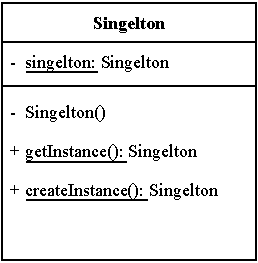
\includegraphics[width=0.25\textwidth]{fig/ainf/Singelton.pdf}
    \caption{UML-Diagramm Singelton}
\end{figure}
Natürlich wird auch ein Zugriffspunkt auf dieses Attribut benötigt.
Implementiert wird dies durch eine weitere statische Methode namens \lstinline{getInstance()}.
Diese Methode ist der einzige Zugriffspunkt auf die Instanz.
\subsubsection{Beispiel}
Das folgende \textit{\autoref{Singelton Code}}, entnommen aus dem \textit{\autoref{subsec:konfiguration}}, zeigt wie Singelton angewendet werden kann.

\lstinputlisting[firstline=22, lastline=38, style=java,caption=Singelton Codebeispiel,label=Singelton Code]{src/data/config/Config.java}

\subsection{Verhaltensmuster Command}\label{subsec:verhaltensmuster-command}
\subsubsection{Beschreibung}
Ziel des Verhaltensmusters Command ist es, den jeweiligen Teilnehmen, welche einen Befehl erzeugt, von dem Teilnehmer der für die Ausführung zuständig ist, zu entkoppeln.
Man kann auch sagen, dass der Teilnehmer, welcher den Befehlsaufruf erzeugt, nicht wissen muss, welcher Teilnehmen den Befehl empfängt oder wo bzw. wann dies geschieht.
Auch kann das tatsächliche Ausführen eines Befehls, aus programmatischer Sicht in einem ganz anderen Thread geschehen, was eine elementare Rolle spielt.
Dieses Verhalten führt zu einer Vereinfachung der Ausführung von komplexeren Tätigkeiten des Programms.
\subsubsection{Struktur}
Das Command-Pattern verfügt meist über verschieden starke Ausprägung.
Im Kern herrscht jedoch immer dasselbe Prinzip, welches in \textit{\autoref{fig:UML-Diagramm Command}} dargestellt wird.
Vorallem die \textbf{Kapselung von Befehlswunsch und Ausführung} steht an erster Stelle.
\begin{figure}[htb!]
    \centering
    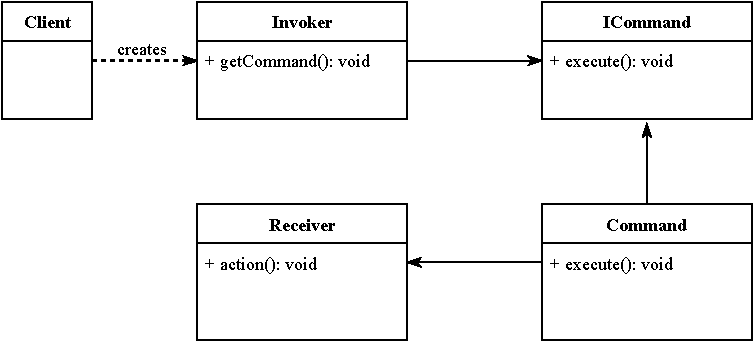
\includegraphics[width=1\textwidth]{fig/ainf/Command.pdf}
    \caption{UML-Diagramm Command}
    \label{fig:UML-Diagramm Command}
\end{figure}
\subsubsection{Beispiel}
\subsection{Entwurfsmuster MVC}\label{subsec:entwurfsmuster-mvc}
\subsubsection{Beschreibung}
Das MVC-Design Pattern, auch Model-View-Controller Design-Pattern, ist eines der weit verbreitetsten Entwurfsmuster.
Es dient zur Strukturierung von Anwendungen und teilt diese in 3 große Bereiche ab, welche strikt voneinander getrennt sind.
Mithilfe dieser Strukturierung fällt es dem Programmierer wesentlich leichter, spätere Änderungen bzw. Erweiterungen am Projekt durchzuführen, da das System nun klar definiert und strukturiert ist.
Auch ist es nun einfacher, parallel an dem Programm zu Arbeiten, denn Ersteller von View und Ersteller des Controllers, also der Berechnungen dahinter, sind nun nicht mehr voneinander abhängig.\\
Jedoch muss bedacht werden, dass Änderungen am Model, direkt an die View weitergegeben werden müssen.
\subsubsection{Struktur}

\begin{enumerate}
    \item \textbf{View}  \\
    Datenrepräsentation\\
    Organisiert alle Kontrollelemente
    \item \textbf{Controller} \\
    Stellt die Verbindung zwischen View und Model her\\
    Verwaltet Benutzerinteraktion und enthält Steuerlogik
    \item \textbf{Model} \\
    Datenrepräsentation\\
    Komplett Abgeschirmt
\end{enumerate}
\begin{figure}[htb!]
    \centering
    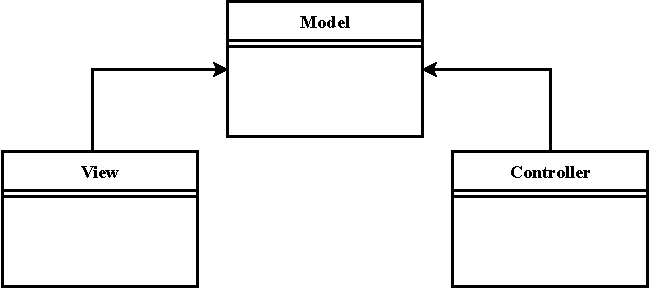
\includegraphics[width=0.8\textwidth]{fig/ainf/ModelViewController.pdf}
    \caption{UML-Diagramm MVC}
    \label{fig:UML-Diagramm MVC}
\end{figure}
\subsection{SceneBuilder}\label{subsec:scenebuilder}
\subsubsection{Beschreibung}
Scenebuilder ist ein umfangreiches GUI-Design-Tool der Firma Gluon.
Verwendet wird es bei Erstellung komplexerer Layouts, denn je komplizierter dieses wird, desto eher stößt man ohne Design-Tool an seine Grenzen.\\\\
Die Verwendung von Tools wie dieses hat mehrere Vorteile.
Einerseits Verbessert sich die Übersichtlichkeit des GUI-Projekts deutlich, da es ab diesem Zeit Zeitpunk möglich ist, den Code hinter der Oberfläche grafisch darzustellen.
Andererseits kann nun, nur mit wenigen Klicks eine für den Endbenutzer ansprechende GUI gebaut werden.\\
Im speziellen hat SceneBuilder weitere wichtige Vorteile wie die direkte Verbindung mit JavaFX und dessen \lstinline{*.fxml} Dateien.
Weiters ist es möglich CSS-Dateien sowie Internationalisierungsdateien einzubinden und diese direkt in SceneBuilder zu verfeinern.
Im wesentlichen ist SceneBuilder, gezeigt in der \autoref{fig:Tool SceneBuilder}, ein performantes Tool und eigent sich optimal für große Projekte wie dieses.
\begin{figure}[htb!]
    \centering
    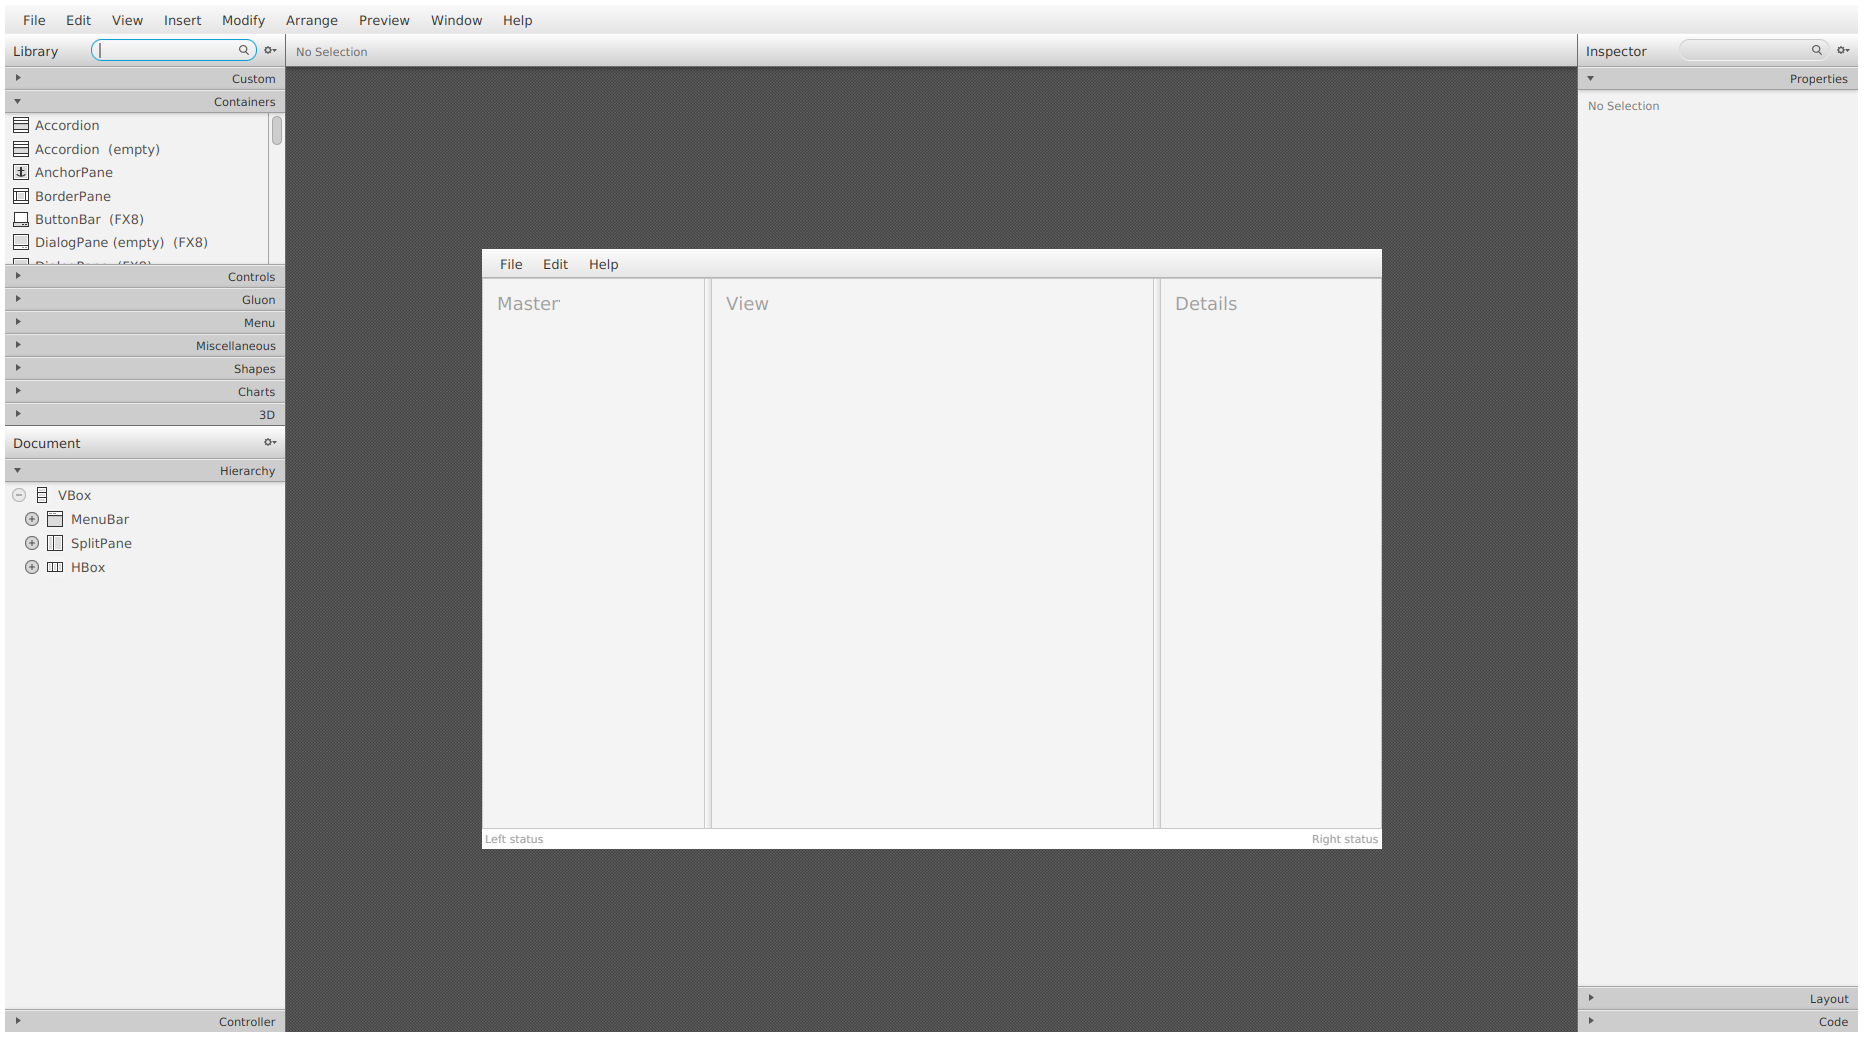
\includegraphics[width=0.8\textwidth]{fig/ainf/SceneBuilder.png}
    \caption{Tool SceneBuilder}
    \label{fig:Tool SceneBuilder}
\end{figure}
\subsubsection{Bibliothek JFoenix}
Sobald nun SceneBuilder als wichtiges Element der Erstellung ausgewählt wurde, kann jetzt ein näherer Blick auf die User-Experience geworfen werden.
Diese sogenannte User-Experience beschreibt, wie der Endbenutzer das Produkt bzw. in unserem Fall die grafische Oberfläche empfindet.
Wird auf diesen Kernpunkt kein Wert gelegt, wird auch niemand erfreut bei der Bedienung sein.\\\\
SceneBuilder bietet bereits einige Grundelemente für Layouts an, doch diese sind nicht ansprechend.
Sie können zwar mir CSS gestaltet werden, dies ist jedoch für alle Elemte schwierig umzusetzten.
Abhilfe schafft dabei die Material-Design Bibliothek von JFoenix.
Diese Bibliothek ist Open-Source und implementiert, wie schon im Namen genannt, Designelemente nach dem von Google entwickelten Material-Design Vorgaben.
Das bedeutet das ohne viel Aufwand, eine höchst ästhetische Oberfläche gebaut werden kann.\\
Anhand der folgenden \autoref{fig:Rendered Button} soll gezeigt werden, wie nun Elemente, gebaut mithilfe der JFoenix Bibliothek, aussehen.
Angewendet werden die Attribute \lstinline{-fx-border-radius: 20pt;}  \lstinline{-fx-background-radius: 20pt;} und \lstinline{-fx-background-color:grey}
\begin{figure}[htb!]
    \centering
    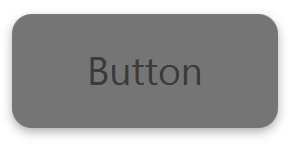
\includegraphics[width=0.5\textwidth]{fig/ainf/RenderedButton.PNG}
    \caption{Gerenderter Button}
    \label{fig:Rendered Button}
\end{figure}
\subsection{Datenformate in Java-FX}\label{subsec:datenformate-in-java-fx}
Im folgenden Kapitel soll auf die Speicherung des Beschreibenden Teils des Layouts eingegangen werden.
Dies geschieht aufgrund des verwendeten GUI-Frameworks nähmlich nicht im Code selbst, sondern in externen Dateien.
Ziel ist es, grundlegende Dinge zu klären und näher zu erläutern.
\subsubsection{XML}
XML(Extensible Markup Language) ist, wie im \autoref{sssec: JavaFX} schon erwähnt, eine Sprache zur Darstellung von Daten in einem von Menschen lesbaren Format.
Damit ist sie also keine Programmiersprache.
Diese XML-Dateien sind zu vergleichen mit normalen Textdokumenten, welche mit einen gewöhnlichen Texteditor geöffnet werden können.

Strukturiert und bezeichnet werden in XML-Dateien die Daten mithilfe von sogenennaten XML-Tags.
Diese Tags stehen in spitzen Klammern und beinhalten den Namen des Datenelements.
Auch ist es notwendig, ein Tag mihilfe eines sogenannten End-Tags zu schließen.
Zwischen diesen Start- bzw. \ End-Tags befindet sich ein Datensatz.
Ein Indikator für ein End-Tag ist ein \lstinline{/}.\\
Anhand der folgenden \autoref{xmlExample} soll gezeigt werden, wie XML-Dateien im inneren aussehen.
% @formatter:off
\begin{lstlisting}[caption=XML-Codebeispiel,label=xmlExample]
<?xml version="1.0" encoding="UTF-8"?>
    <email>
        <to>Person1</to>
        <from>Person2</from>
        <heading>Test-Header</heading>
        <body>This is a body :)</body>
    </email>
\end{lstlisting}
% @formatter:on

\subsubsection{FXML}
FXML ist ein auf XML basierendes Datenformat, welches hauptsächlich bei der Erstellung von JavaFX Anwendungen angewendet wird.
Da hier die Trennung von GUI- und Programmcode vollzogen wurde, kann erst mithilfe des von Oracle entwickelte Formats ein Layout nach dem MVC -Pattern gebaut werden.\\\\
Die Struktur und Syntax von FXML Dateien ähnelt der von XML-Dateien.
So werden auch Start- und End-Tags verwendet.
Ein wesentlicher Unterschied ist jedoch bei der Groß-/Kleinschreibung ersichtlich.
Beginnen in FXML-Dateien Elemente mit einem Großbuchstaben, werden diese als Objektdeklarationen behandelt.
Infolgedessen erkennt der FXML-Loader, welcher diese \lstinline{*.fxml} ins Programm lädt, diese Objektdeklarationen nimmt eine dementsprechende Objektbildungen vor.
Sobald diese jedoch mit einem Kleibuchstaben beginnen, definieren sie Eigenschaften.
Eine weitere Besonderheit ist, dass es möglich ist, Import-Anweisungen durchzuführen.
Dies können mithilfe des Tags \lstinline{<?import ... ?>} ausgeführt werden.\\
\begin{lstlisting}[caption=FXML-Codebeispiel,label=fxmlExample]
<?xml version="1.0" encoding="UTF-8"?>
<?import javafx.scene.layout.VBox?>
<?import javafx.scene.control.Label?>

<VBox>
    <children>
    <Label text="Hello ReShuffled :)"/>
    </children>
</VBox>
\end{lstlisting}

\subsubsection{CSS}
Bei der Verfolgung von Designzielen spielt auch CSS(Cascading Style Sheet) eine wichtige Rolle.
\subsection{Datenformat JSON}\label{subsec:json}

\subsubsection{Beschreibung}

\subsubsection{Bibliothek GSON}

\section{Backend-Programmierung}\label{sec:backend-programmierung}
\subsection{Kommunikation - serielle Schnittstelle}\label{subsec:kommunikation---serielle-schnittstelle}
\subsubsection{Konzept}
Um erfolgreich Daten zwischen dem Raspberry PI 3B+ und der Platine, welche die Ansteuerung sämtlicher Komponenten übernimmt, zu übertragen, wird ein Kommunikationsprotokoll benötigt.
Dieses Protokoll stellt im engsten Sinne eine Vereinbarung dar, wie die Datenübertragung zwischen zwei oder mehreren Parteien abläuft.
Anforderungen an dieses Protokoll sollen sein:
\begin{enumerate}
    \item einfache Integration in die Zielsysteme
    \item erweiterbarkeit des Protokolls mit geringem Arbeitsaufwand
    \item hohe Sicherheit gegenüber Übertragungsfehler
    \item schnelle Fehlererkennung sowie Fehlerbehebung
\end{enumerate}
Neben standartisierten Protokollen wie Modbus, Feldbus oder CAN-Bus gibt es die Möglichkeit selbst ein sogenanntes propretäres Übertragungsprotokoll zu kreieren.
Dies ist in unserem Fall nötig, um alle Anforderungen abzudecken.
Basierend auf dem Master - Slave Prinzip, wobei der Rasperry PI den Master und die Ansteuerplatine den Slave darstellt, soll ein abgewandeltes Modbus ASCII Protokoll umgesetzt werden.

Zusätzlich soll, um die Anforderung des einfachen Fehlerhandlings zu erfüllen, ein Simulator ausprogrammiert werden, welcher beim Start auf Softwarebebene, den Platz des Slaves bzw. der Ansteuerplatine einnimmt.
Der Startvorgang des Simulators soll mit einer einfachen Modifizierung der Konfigurationsdatei vonstatten gehen.
Die folgende Grafik soll die schematisch die Geräteauswahl darstellen.
\begin{figure}[H]
    \centering
    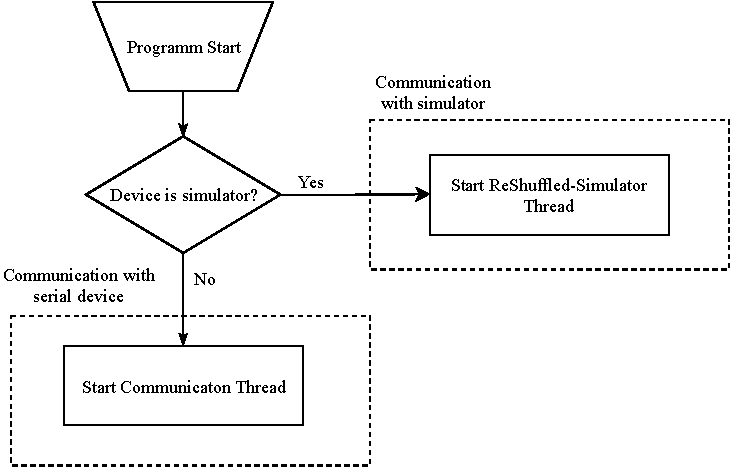
\includegraphics[width=0.8\textwidth]{fig/ainf/DeviceSelection}
    \caption{Schematische Darstellung der Geräteauswahl}
\end{figure}
\begin{enumerate}
    \item Einzelbitfehler (1 Bit verändert)
    \item Burstfehler (ganze Folge von Bits verändert)
\end{enumerate}
\subsubsection{Übertragungsprotokoll}
\begin{table}[htb!]
    \centering
    \begin{tabular}{|
    >{\columncolor[HTML]{FFFFFF}}l |
    >{\columncolor[HTML]{FFFFFF}}l |
    >{\columncolor[HTML]{FFFFFF}}l |
    >{\columncolor[HTML]{FFFFFF}}l |
    >{\columncolor[HTML]{FFFFFF}}l |}
        \hline
        \textbf{Doppelpunkt :} & \textbf{Daten (ASCII)} & \textbf{Trennzeichen \#} & \textbf{CRC32-Prüfsumme} & \textbf{Semicolon \textbackslash{}n} \\ \hline
        8-Bit & 16-Bit & 8-Bit & 32-Bit & 8-Bit                                \\ \hline
    \end{tabular}
    \caption{Visualisierung des Datenakets}
\end{table}
Das verbindugslose Protokoll basiert, wie in der Konzeptbeschreibung bereits erwähnt, auf dem Master-Slave Prinzip.
Außerdem erfolgt die Datenübertragung rein textuell wobei nur Großbuchstaben verwendet werden dürfen.\\\\
Wie aus der oben dargestellten Tabelle zu entnehmen, ist der Aufbau eines Frames klar definiert.
Der eindeutige Start des Datenpakets, welcher mit einem Doppelpunkt (:) eingeleitet wird, sowie das ebenfalls eindeutige Ende, umgesetzt mit einem Line Feed Character (), bringt eindeutige Vorteile mit sich.
Im Gegensatz zu anderen Protokollen wie z.B. Modbus RTU, muss hier nicht auf das Ende des Pakets "gewartet" werden. Dies führ oft zu Einbußen im Bereich der Performance und ist für uns nicht zielführend.\\\\
Gefolgt von dem Startzeichen folgen nun die Daten.
Diese beinhalten eindeutig definierte Zecichenfolgen, welche verwendet werden um verschiedenste Zustände der Ansteuerplatine auszuführen.
Diese Um auch hier zu wissen, wo sich das der Nutzdaten befindet, schließt das Trennzeichen () diese ab.\\\\
Um nun die Integrität, also die Korrektheit der Daten bei einer Übertragung zu überprüfen, wird im nächsten Schritt eine Prüfsumme verwendet.
Ziel dieser ist es, anhand der Nutzdaten einen Wert zu bilden, welcher danach vom Sender im Frame gespeichert bzw übertragen wird.
Der Empfänger berechnet nun mit dem selben Verfahren die Prüfsumme aus den empfangenen Daten und vergleicht diese mit der Übertragenen Prüfsumme des Senders.
Sind beide Prüfsummen identisch, war die Übertragung erfolgreich und die Daten sind mit großer Wahrscheinlichkeit korrekt.
Stimmen diese nicht überein liegt ein Fehler vor.
Die wichtigsten Arten von Übertragungsfehlern sind:
Neben einfachen Verfahren wie z.B. dem Paritätsbit-Verfahren gibt es auch Komplexere. Die zyklische Redundanzprüfung, auch CRC genannt, ist eines davon.
Sie ist realtiv einfach zu realisieren und dennoch wirkungsvoll.
Wichtig beim CRC-Verfahren ist, dass beide Teilnehmen, also Sender und Empfänger, das selbe Generator-Polynom verwenden. Der Grad des Generatorpolyoms beträgt in unserem Fall 32 (CRC-32).
\subsubsection{Request- und Responsehandling}

\subsection{Kommunikation - Debugging-Simulator}\label{subsec:kommunikation---debugging-simulator}
\subsubsection{Konzept}
\subsubsection{Datenaustausch}
\subsubsection{Verarbeitung ankommender Daten}
\subsection{Logging}
\subsubsection{Konzept}
\subsubsection{Integration in das Programm}
\subsection{Konfiguration}\label{subsec:konfiguration}
\subsubsection{Konzept}
\subsubsection{Datenmodelle}
\subsubsection{Verwahrung am Zielsystem}

\subsection{Statistiken}
\subsubsection{Konzept}
\subsubsection{Datenmodelle}
\subsubsection{Verwahrung am Zielsystem}

\subsection{Controllerklassen}
\subsubsection{Grundlagen}
\subsubsection{StartupController}
\subsubsection{MainController}
\subsubsection{HomeController}
\subsubsection{StatsController}
\subsubsection{About- und HelpController}


\section{Frontend-Programmierung}
\subsection{Designkonzept}



\begin{lstlisting}[style=java,caption=Java Codebeispiel,label=Model]
public class Model extends Observable{
private int counter;
public Model() {
}
public int getCounter() {
return countDown;
}
public void increment() {
if (counter > 0) {
counter++;
}
notifyObservers();
}
\end{lstlisting}

\begin{lstlisting}[style=java,caption=Die Klasse View,label=View]
public class View implements Observer {
private Model model;
private Stage stage;
private Label label;
private Button countButton;
public View(Model model, Stage stage) {
this.model = model;
this.stage = stage;
label = new Label("Counter: " + model.getCounter());
btIncrement = new Button("Increment by 1");
stage.setScene(new Scene(new VBox(label, countButton)));
model.addObserver(this);
}
@Override
public void update(Observable o, Object arg) {
label.setText("Counter: " + model.getCounter());
\end{lstlisting}
\subsection{Utility Klassen}
\subsubsection{AlertUtil}
\subsubsection{GuiUtil}
\subsection{Implementierung von CSS}
\subsubsection{StartupCSS}
\subsubsection{HomeCSS}
\subsection{Internationalisierung}
\subsubsection{Gründe der Umsetzung}
\subsubsection{Integration in das Interface}
\subsubsection{Ressourcen Manager}
\subsubsection{Resource Utility}
\subsubsection{Bereitgestellte Ressources Bundles}

\section{Hardwarenahe-Programmierung}
\subsection{Einrichtung des Mikrocontrollers}
\subsection{Konzept und Ablaufdiagramm zur Kartenausgabe}
\subsection{Request- und Responsehandling}
\section{Teilaufbau}
\subsection{Auswahl des Zielsystems}
\subsubsection{Arduino}
\subsubsection{Raspberry PI}
\subsection{Auswahl des Displays}
\subsection{Montage und Testaufbau}
\subsection{Konfiguration des Zielsytsems}
\subsubsection{Betriebssystem}
\subsubsection{Speichermedium}
\subsubsection{Touchpanel}
\subsubsection{SSH und SFTP}
\subsubsection{Autostart realisiert durch Services}

\section{Probleme - Verbesserungsmöglichkeiten - Zusammenfassung}
\subsection{Probleme}
\subsubsection{Probleme bei der Implementierung von JavaFX}
\subsubsection{Kommunikation zwischen Controllern}
\subsection{Verbesserungsmöglichkeiten}
\subsubsection{Online Update-Möglichkeit der Software}
\subsubsection{Smartphone-Interface zum Zählen der Punkte}
\subsection{Zusammenfassung}